\documentclass{article}

\usepackage{graphicx}
\usepackage{float}
\usepackage{booktabs}
\usepackage{makecell}
\usepackage{listings}

\usepackage{color}
\definecolor{lightgray}{gray}{0.9}

\lstset{
    showstringspaces=false,
    basicstyle=\ttfamily,
    keywordstyle=\color{blue},
    commentstyle=\color[grey]{0.6},
    stringstyle=\color[RGB]{255,150,75}
}

\newcommand{\inlinecode}[2]{{\lstinline[language=#1]$#2$}}

\renewcommand{\cellalign}{l}

\lstset{
    language=Java,
    basicstyle=\small\sffamily,
    numbers=left,
    numberstyle=\tiny,
    frame=tb,
    tabsize=4,
    columns=fixed,
    showstringspaces=false,
    showtabs=false,
    keepspaces,
    commentstyle=\color{red},
    keywordstyle=\color{blue}
}

\title{Applicazione per la gestione del cibo}

\date{2024-05-10}

\author{Saverio Napolitano}

\begin{document}

\maketitle

\pagenumbering{gobble}

\tableofcontents

\newpage

\pagenumbering{arabic}

\section{Introduzione}

Expiration Date è un'applicazione nata per permettere la gestione completa di tutto ciò che riguarda i prodotti alimentari; con essa è infatti possibile gestire gli aspetti relativi:
\begin{itemize}

  \item alla lista della spesa (prodotti che si desidera acquistare)
  \item alla dispensa (prodotti già posseduti)
  \item alle ricette
  
\end{itemize}

\section{Specifica dei requisiti}

Nelle sezioni seguenti verranno illustrati i principali requisiti che l'applicazione si pone come obiettivo di soddisfare.

\subsection{Requisiti funzionali}

Essi descrivono le funzionalità che il sistema deve offrire, intendendo con questo sia le operazioni che l'applicazione svolge sia le interazioni che la stessa ha con l'utente o con altri sistemi esterni con cui si interfaccia.

\begin{table}[H]
    \begin{flushleft}
      \begin{tabular}{l|l}
        \toprule
        \textbf{RF01} & \textbf{Aggiunta alimenti in dispensa}\\
        \midrule
        Input & Dati alimento acquistato - nome alimento, data di scadenza, quantità\\
        Processo & Memorizzazione su lista e database degli alimenti\\
        Output & Visualizzazione alimenti\\
        \bottomrule
      \end{tabular}
    \end{flushleft}
\end{table}

\begin{table}[H]
    \begin{flushleft}
      \begin{tabular}{l|l}
        \toprule
        \textbf{RF01.1} & \textbf{Generazione notifica scadenza alimento}\\
        \midrule
        Input & Aggiunta di un prodotto alla dispensa\\
        Processo & Si crea l’avviso su calendario relativo alla scadenza del prodotto\\
        Output & Aggiunta dell’avviso sul calendario dell’utente\\
        \bottomrule
      \end{tabular}
    \end{flushleft}
\end{table}

\begin{table}[H]
    \begin{flushleft}
      \begin{tabular}{l|l}
        \toprule
        \textbf{RF02} & \textbf{Rimozione alimenti in dispensa}\\
        \midrule
        Input & Click su pulsante “Delete”\\
        Processo & Eliminazione alimento dalla lista e dal database\\
        Output & Visualizzazione lista aggiornata\\
        \bottomrule
      \end{tabular}
    \end{flushleft}
\end{table}

\begin{table}[H]
    \begin{flushleft}
      \begin{tabular}{l|l}
        \toprule
        \textbf{RF02.1} & \textbf{Rimozione avviso su calendario}\\
        \midrule
        Input & Rimozione prodotto dalla dispensa\\
        Processo & Cancellazione avviso su calendario\\
        Output & Rimozione avviso su calendario\\
        \bottomrule
      \end{tabular}
    \end{flushleft}
\end{table}

\begin{table}[H]
    \begin{flushleft}
      \begin{tabular}{l|l}
        \toprule
        \textbf{RF03} & \textbf{Ordinamento prodotti dispensa per nome}\\
        \midrule
        Input & Click sulla colonna “Product”\\
        Processo & Ordinamento prodotti in modo crescente o decrescente in base al nome\\
        Output & Visualizzazione prodotti ordinati\\
        \bottomrule
      \end{tabular}
    \end{flushleft}
\end{table}

\begin{table}[H]
    \begin{flushleft}
      \begin{tabular}{l|l}
        \toprule
        \textbf{RF04} & \textbf{Ordinamento prodotti in dispensa per data di scadenza}\\
        \midrule
        Input & Click sulla colonna “Expiration Date”\\
        Processo & Ordinamento prodotti in modo crescente o decrescente in base alla data di scadenza\\
        Output & Visualizzazione prodotti ordinati\\
        \bottomrule
      \end{tabular}
    \end{flushleft}
\end{table}

\begin{table}[H]
    \begin{flushleft}
      \begin{tabular}{l|l}
        \toprule
        \textbf{RF05} & \textbf{Modifica nome alimento in dispensa}\\
        \midrule
        Input & Doppio click sul nome alimento e inserimento nuovo nome\\
        Processo & Aggiornamento nome alimento in memoria e in database\\
        Output & Visualizzazione alimento con nome aggiornato\\
        \bottomrule
      \end{tabular}
    \end{flushleft}
\end{table}

\begin{table}[H]
    \begin{flushleft}
      \begin{tabular}{l|l}
        \toprule
        \textbf{RF06} & \textbf{Modifica dati alimento in dispensa}\\
        \midrule
        Input & Doppio click su data di scadenza e modifica dati\\
        Processo & \makecell{Si apre una nuova finestra che consente la modifica dei dati dell’alimento; \\ Aggiornamento dati alimento in memoria e in database}\\
        Output & Visualizzazione alimenti aggiornati\\
        \bottomrule
      \end{tabular}
    \end{flushleft}
\end{table}

\begin{table}[H]
    \begin{flushleft}
      \begin{tabular}{l|l}
        \toprule
        \textbf{RF06.1} & \textbf{Modifica avviso calendario}\\
        \midrule
        Input & Modifica data di scadenza e/o nome prodotto\\
        Processo & Aggiornamento data di scadenza e/o nome prodotto sul calendario\\
        Output & Visualizzazione calendario aggiornato\\
        \bottomrule
      \end{tabular}
    \end{flushleft}
\end{table}

\begin{table}[H]
    \begin{flushleft}
      \begin{tabular}{l|l}
        \toprule
        \textbf{RF07} & \textbf{Aggiunta alimenti in lista della spesa}\\
        \midrule
        Input & Nome alimento da acquistare\\
        Processo & Salvataggio su memoria e database della lista della spesa\\
        Output & Visualizzazione lista della spesa\\
        \bottomrule
      \end{tabular}
    \end{flushleft}
\end{table}

\begin{table}[H]
    \begin{flushleft}
      \begin{tabular}{l|l}
        \toprule
        \textbf{RF08} & \textbf{Rimozione alimenti in lista della spesa}\\
        \midrule
        Input & Click su pulsante “Delete”\\
        Processo & Eliminazione alimento dalla lista e dal database della lista della spesa\\
        Output & Visualizzazione aggiornata lista della spesa\\
        \bottomrule
      \end{tabular}
    \end{flushleft}
\end{table}

\begin{table}[H]
    \begin{flushleft}
      \begin{tabular}{l|l}
        \toprule
        \textbf{RF09} & \textbf{Alimento in lista della spesa comprato}\\
        \midrule
        Input & Utente clicca sulla checkbox che segnala l’acquisto di un elemento nella lista della spesa\\
        Processo & Viene azionata la stessa procedura che implementa il requisito \textbf{RF01}\\
        Output & Visualizzazione alimenti e aggiornamento lista della spesa\\
        \bottomrule
      \end{tabular}
    \end{flushleft}
\end{table}

\begin{table}[H]
    \begin{flushleft}
      \begin{tabular}{l|l}
        \toprule
        \textbf{RF10} & \textbf{Pulizia lista della spesa}\\
        \midrule
        Input & Click sul pulsante “Clear” della lista della spesa\\
        Processo & Rimozione dalla lista della spesa, sia in memoria che in database, degli alimenti già acquistati\\
        Output & Visualizzazione lista della spesa aggiornata\\
        \bottomrule
      \end{tabular}
    \end{flushleft}
\end{table}

\begin{table}[H]
    \begin{flushleft}
      \begin{tabular}{l|l}
        \toprule
        \textbf{RF11} & \textbf{Visualizzazione ricette memorizzate}\\
        \midrule
        Input & \makecell{Click sul pulsante “Recipe” nella dispensa e all’interno della schermata “Recipe” attraverso \\ le frecce di navigazione è possibile passare da una ricetta alla successiva}\\
        Processo & Caricamento dal database delle ricette\\
        Output & Visualizzazione ricette\\
        \bottomrule
      \end{tabular}
    \end{flushleft}
\end{table}

\begin{table}[H]
    \begin{flushleft}
      \begin{tabular}{l|l}
        \toprule
        \textbf{RF12} & \textbf{Aggiunta ricette}\\
        \midrule
        Input & \makecell{Click su pulsante “Add” e inserimento dati ricetta - titolo, durata, numero porzioni, \\ categoria, lista dei tag, lista ingredienti, procedimento ricetta}\\
        Processo & Salvataggio su database e in memoria della ricetta\\
        Output & Visualizzazione ricetta\\
        \bottomrule
      \end{tabular}
    \end{flushleft}
\end{table}

\begin{table}[H]
    \begin{flushleft}
      \begin{tabular}{l|l}
        \toprule
        \textbf{RF13} & \textbf{Modifica dati ricetta}\\
        \midrule
        Input & Modifiche su dati ricetta\\
        Processo & Salvataggio in memoria e database dei dati della ricetta aggiornati\\
        Output & Visualizzazione ricetta aggiornata\\
        \bottomrule
      \end{tabular}
    \end{flushleft}
\end{table}

\begin{table}[H]
    \begin{flushleft}
      \begin{tabular}{l|l}
        \toprule
        \textbf{RF14} & \textbf{Controllo disponibilità ingredienti}\\
        \midrule
        Input & Visualizzazione ricetta o modifica della stessa\\
        Processo & Confronto fra i prodotti in dispensa e gli ingredienti necessari per la ricetta\\
        Output & Visualizzazione ingredienti disponibili e non disponibili per la ricetta attuale\\
        \bottomrule
      \end{tabular}
    \end{flushleft}
\end{table}

\begin{table}[H]
    \begin{flushleft}
      \begin{tabular}{l|l}
        \toprule
        \textbf{RF15} & \textbf{Eliminazione ricetta}\\
        \midrule
        Input & Click sul pulsante “Delete” nella schermata delle ricette\\
        Processo & Rimozione da memoria e database della ricetta attuale\\
        Output & \makecell{Visualizzazione di un’altra ricetta o aggiunta di una nuova ricetta vuota se non ci sono più \\ ricette}\\
        \bottomrule
      \end{tabular}
    \end{flushleft}
\end{table}

\begin{table}[H]
    \begin{flushleft}
      \begin{tabular}{l|l}
        \toprule
        \textbf{RF16} & \textbf{Import ricette da file}\\
        \midrule
        Input & File contenente una lista di ricette\\
        Processo & Salvataggio in memoria e database dei dati della ricette sul file importato\\
        Output & Visualizzazione ricette importate\\
        \bottomrule
      \end{tabular}
    \end{flushleft}
\end{table}

\begin{table}[H]
    \begin{flushleft}
      \begin{tabular}{l|l}
        \toprule
        \textbf{RF17} & \textbf{Export ricette su file}\\
        \midrule
        Input & Click su pulsante “Export”\\
        Processo & Creazione di un file su cui sono memorizzate le ricette presenti in database\\
        Output & File con lista delle ricette\\
        \bottomrule
      \end{tabular}
    \end{flushleft}
\end{table}

\subsection{Requisiti non funzionali}

Essi descrivono le caratteristiche che l'applicazione deve avere che non sono direttamente collegate alle operazioni che esegue.

\begin{table}[H]
  \begin{flushleft}
    \begin{tabular}{l|l}
      \toprule
      \textbf{RNF01} & \textbf{Tempi di risposta}\\
      \midrule
      Descrizione & \makecell{Il software dovrà garantire tempi di risposta minimi per tutte le operazioni,\\ consentendo agli utenti di interagire con l'applicazione in tempo reale}\\
      \bottomrule
    \end{tabular}
  \end{flushleft}
\end{table}

\begin{table}[H]
  \begin{flushleft}
    \begin{tabular}{l|l}
      \toprule
      \textbf{RNF02} & \textbf{Database (salvataggio dei dati)}\\
      \midrule
      Descrizione & \makecell{L'applicazione dovrà utilizzare un sistema di database affidabile e sicuro per garantire la \\ persistenza dei dati relativi ai prodotti nella dispensa, ai prodotti presenti nella lista della \\ spesa e alle ricette}\\
      \bottomrule
    \end{tabular}
  \end{flushleft}
\end{table}

\begin{table}[H]
  \begin{flushleft}
    \begin{tabular}{l|l}
      \toprule
      \textbf{RNF03} & \textbf{Portabilità}\\
      \midrule
      Descrizione & \makecell{L'applicazione deve essere progettata in modo da essere compatibile sia con i sistemi \\ Android che iOS}\\
      \bottomrule
    \end{tabular}
  \end{flushleft}
\end{table}

\begin{table}[H]
  \begin{flushleft}
    \begin{tabular}{l|l}
      \toprule
      \textbf{RNF04} & \textbf{Integrazione con servizi di terze parti}\\
      \midrule
      Descrizione & Il sistema deve essere in grado di interagire con il calendario predefinito dell'utente\\
      \bottomrule
    \end{tabular}
  \end{flushleft}
\end{table}

\section{Descrizione del progetto}

Per questa descrizione si farà riferimento alla versione desktop dell'applicazione.

Il software presenta due schermate principali:

\begin{itemize}

  \item una per la gestione della dispensa e della lista della spesa
  \item una per la gestione delle ricette

\end{itemize}

\begin{figure}[H]
    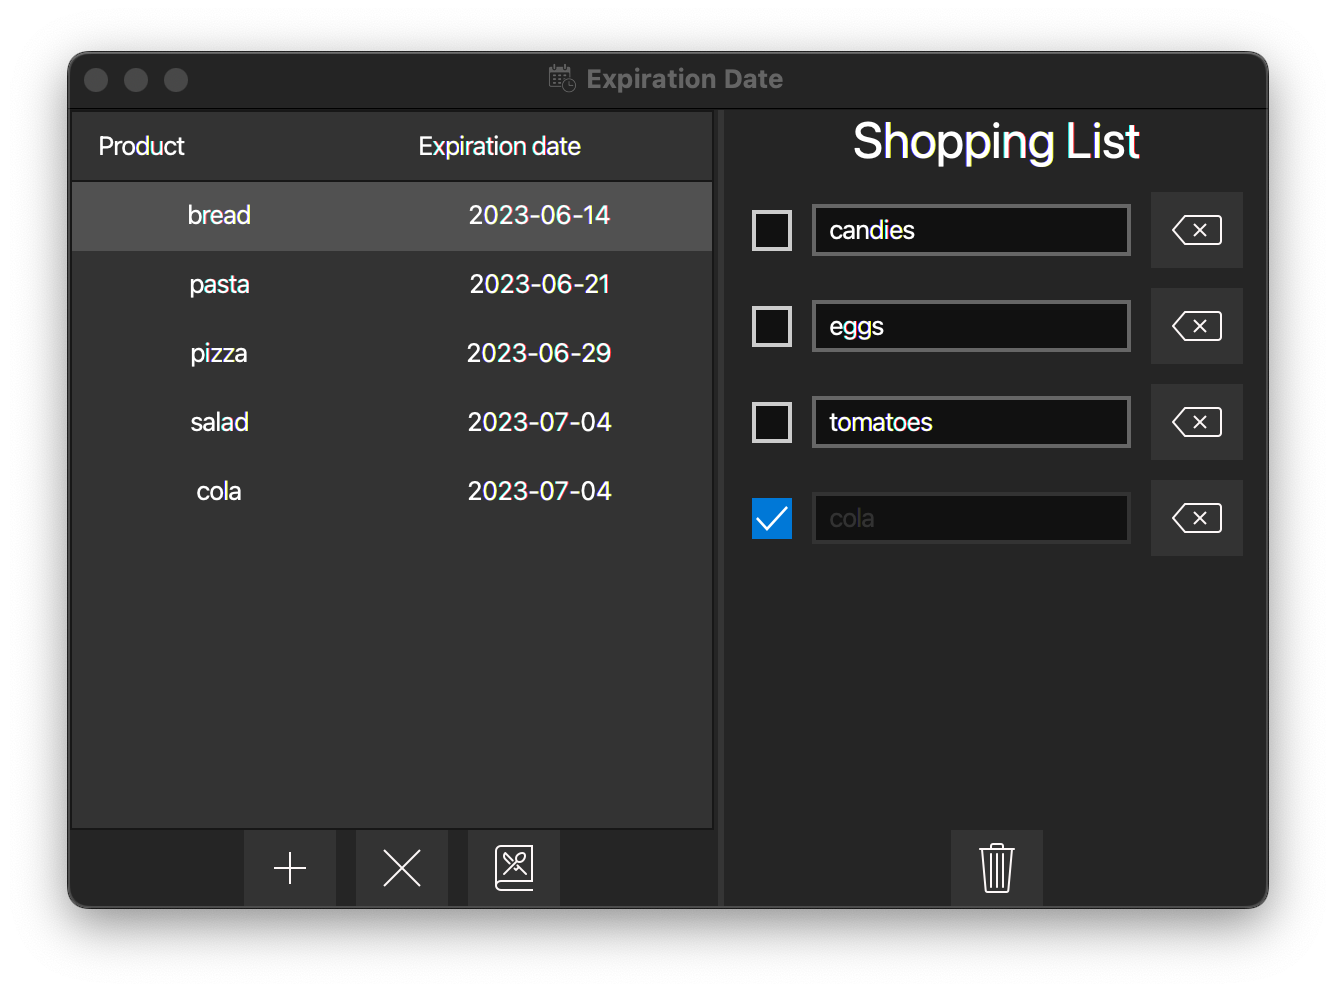
\includegraphics[width=\linewidth]{images/main-view.png}
    \caption{Finestra per la gestione di dispensa e lista della spesa.}
    \label{fig:mainview}
\end{figure}

La schermata per la gestione della dispensa e della lista della spesa si divide in due parti:

\begin{itemize}
  \item la parte di sinistra permette di aggiungere prodotti alla dispensa, eliminare prodotti dalla dispensa, modificare i dati di un prodotto o passare alla schermata delle ricette
  \begin{itemize}
    \item nel caso si desideri modificare i dati di un prodotto comparirà una schermata apposita per la modifica

    \begin{figure}[H]
        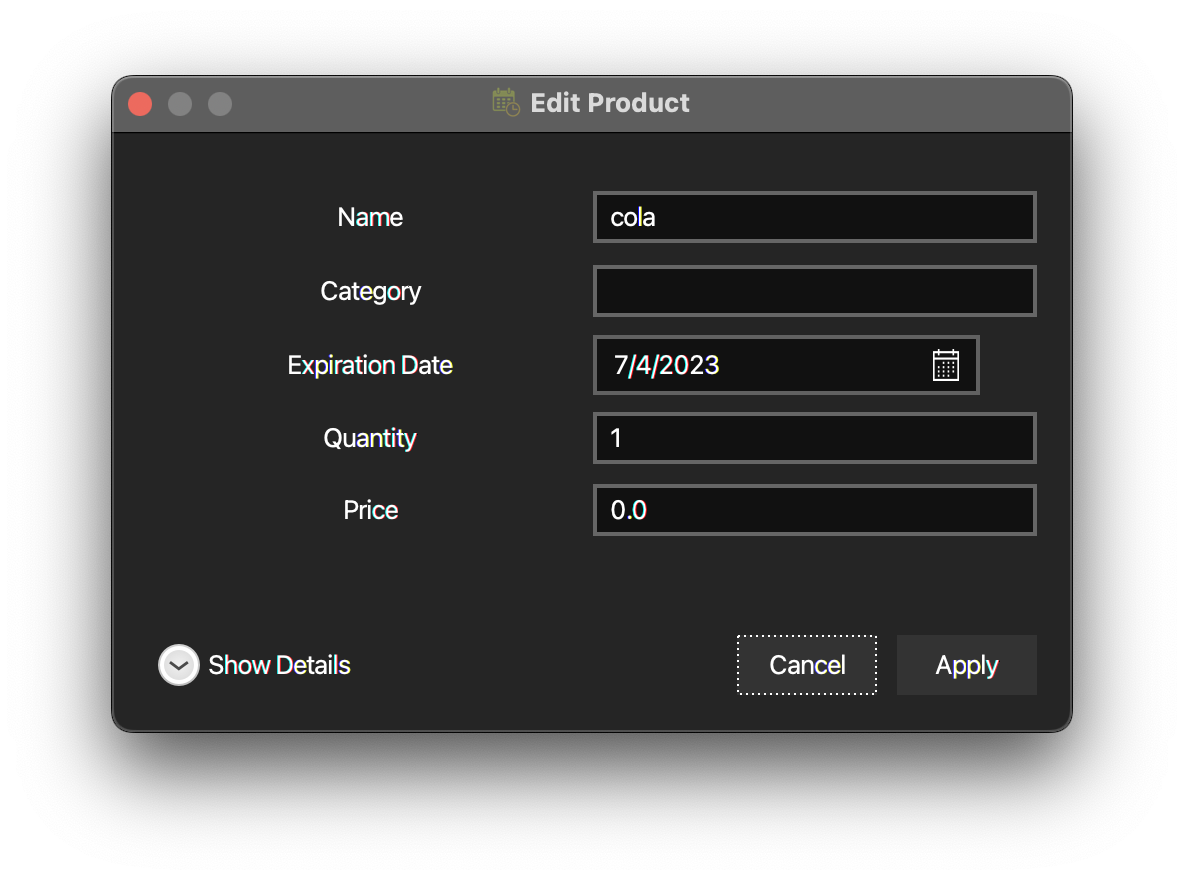
\includegraphics[width=\linewidth]{images/edit-product.png}
        \caption{Finestra per la modifica dei dati del prodotto.}
        \label{fig:editproduct}
    \end{figure}

  \end{itemize}
  \item la parte di destra permette di aggiungere prodotti alla lista della spesa, eliminare prodotti dalla lista della spesa, contrassegnare un prodotto della lista della spesa come "acquistato" (e aggiungerlo in automatico alla dispensa) e rimuovere tutti i prodotti contrassegnati come acquistati
\end{itemize}

La schermata per la gestione delle ricette permette di navigare tra le ricette con le apposite frecce, aggiungere una ricetta, rimuovere una ricetta, modificare i dati di una ricetta, importare ed esportare liste di ricette.

\begin{figure}[H]
    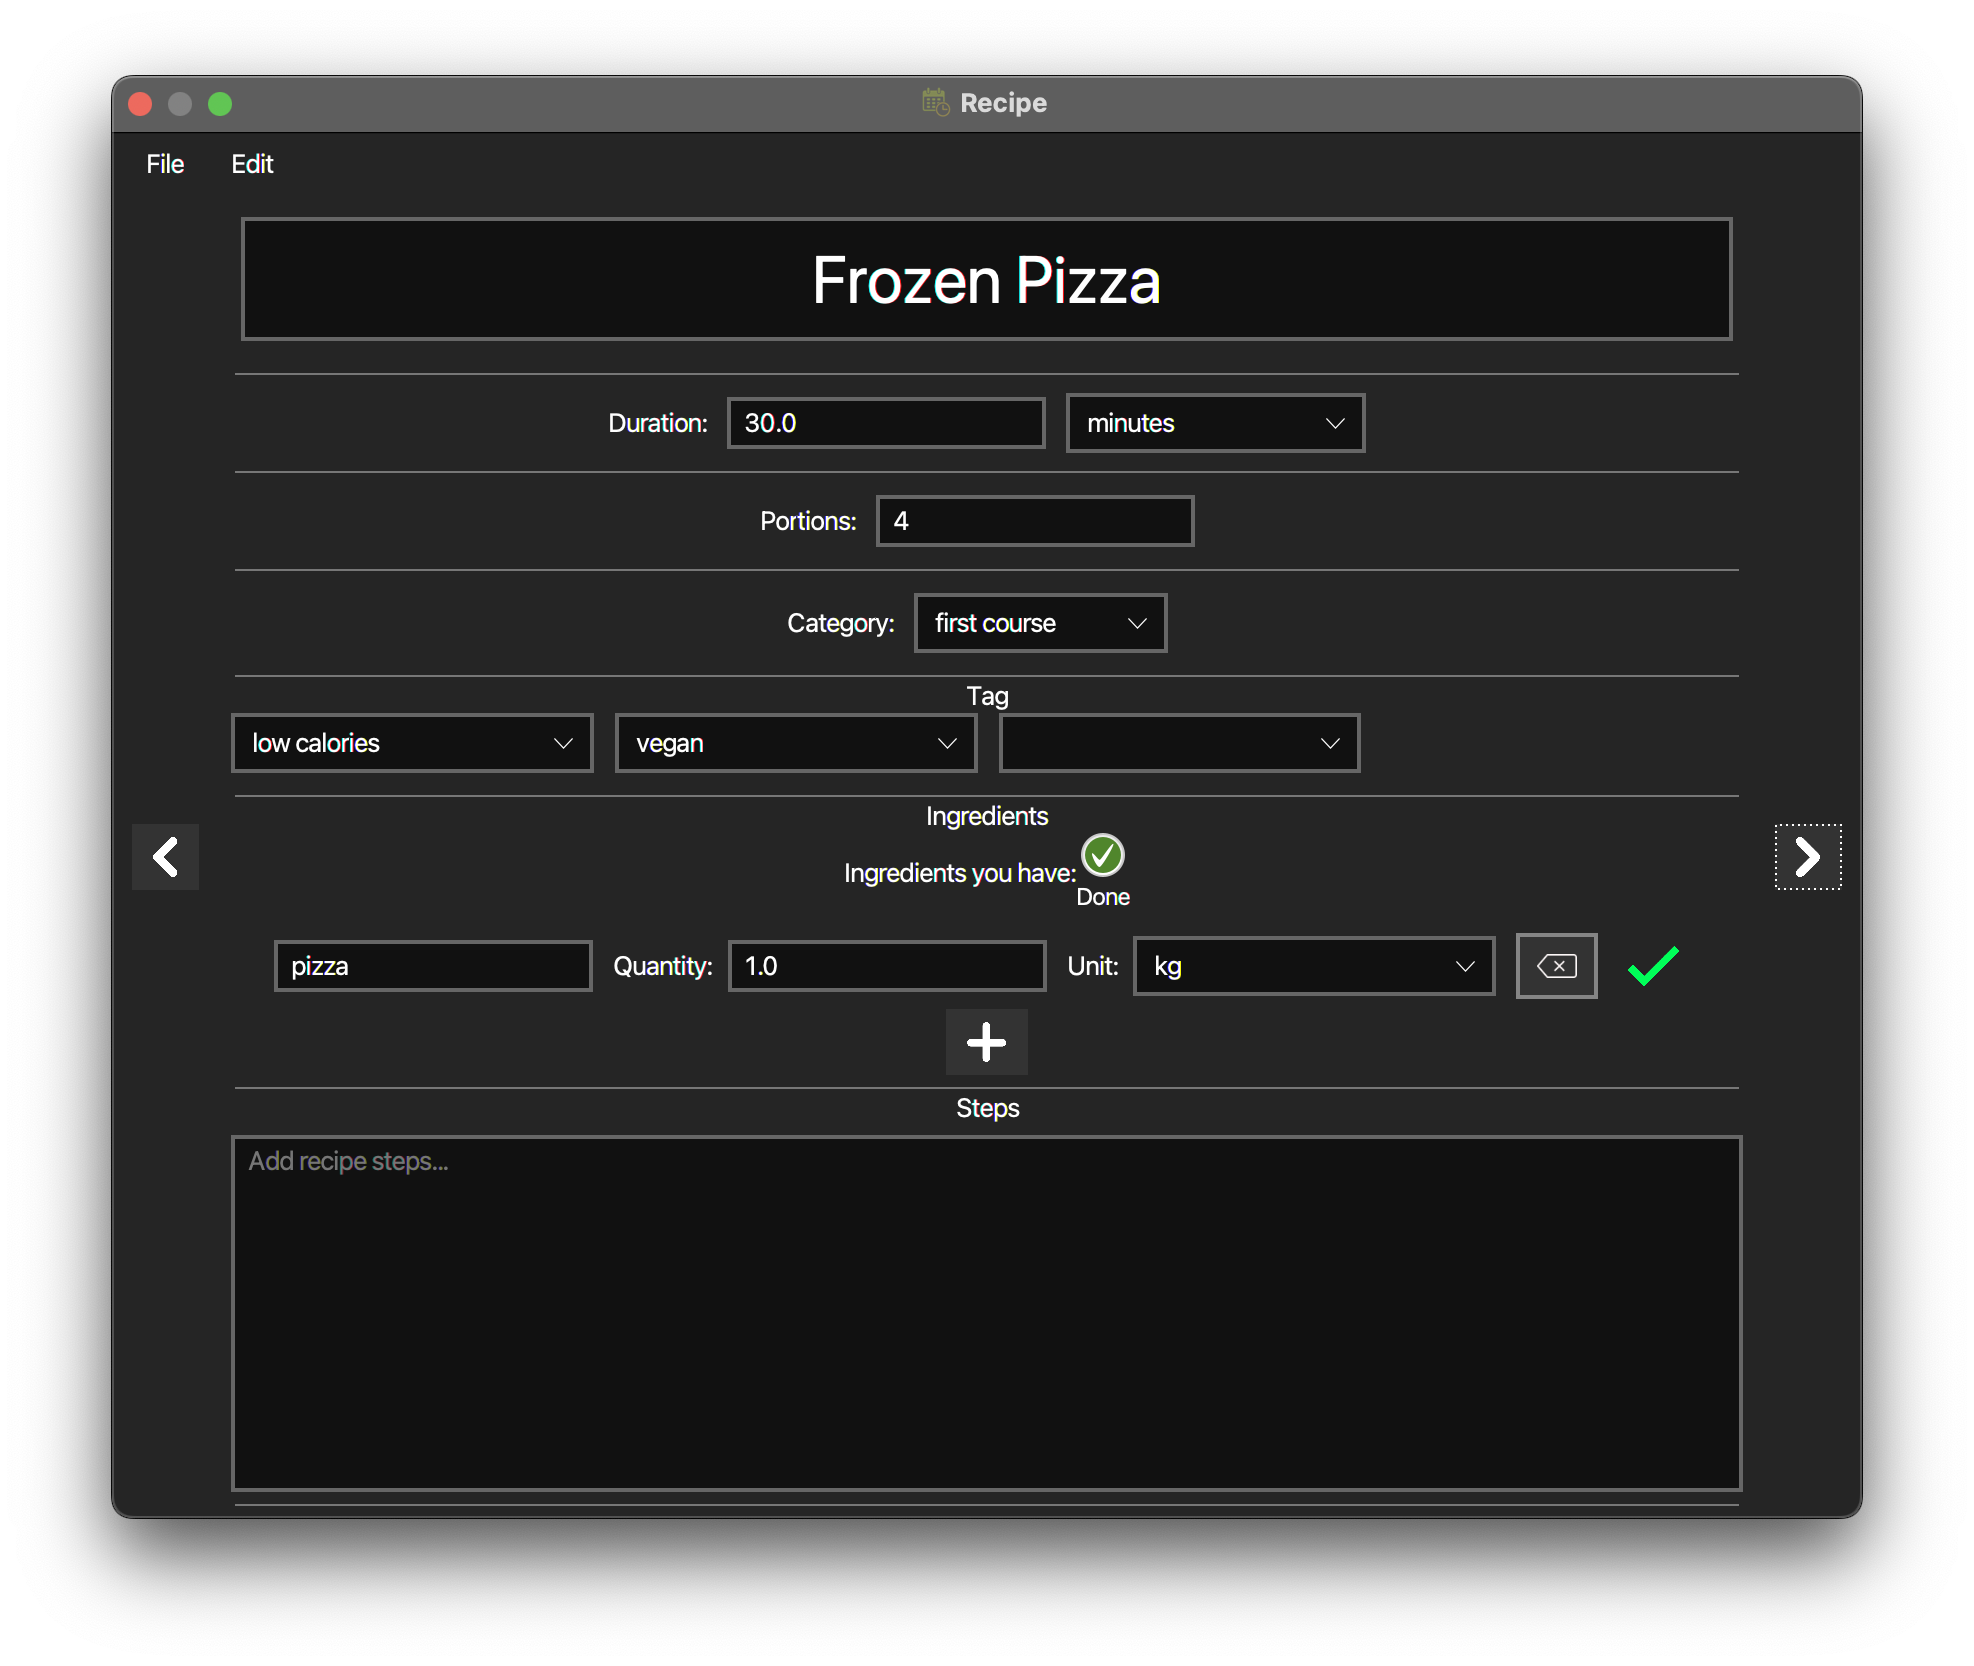
\includegraphics[width=\linewidth]{images/recipe-view.png}
    \caption{Finestra per la gestione delle ricette.}
    \label{fig:recipeview}
\end{figure}

\section{UML}

I diagrammi UML permettono di descrivere graficamente l'applicazione sotto vari punti di vista, garantendo la comprensione del funzionamento del software, delle esigenze che esso soddisfa e delle relazioni che intercorrono fra i suoi componenti.

\subsection{Use case diagram}

Lo use case diagram permette di identificare gli attori che interagiscono col sistema e le attività che essi possono svolgere. Lo scopo è descrivere le principali funzionalità del software.

\begin{figure}[h!]
    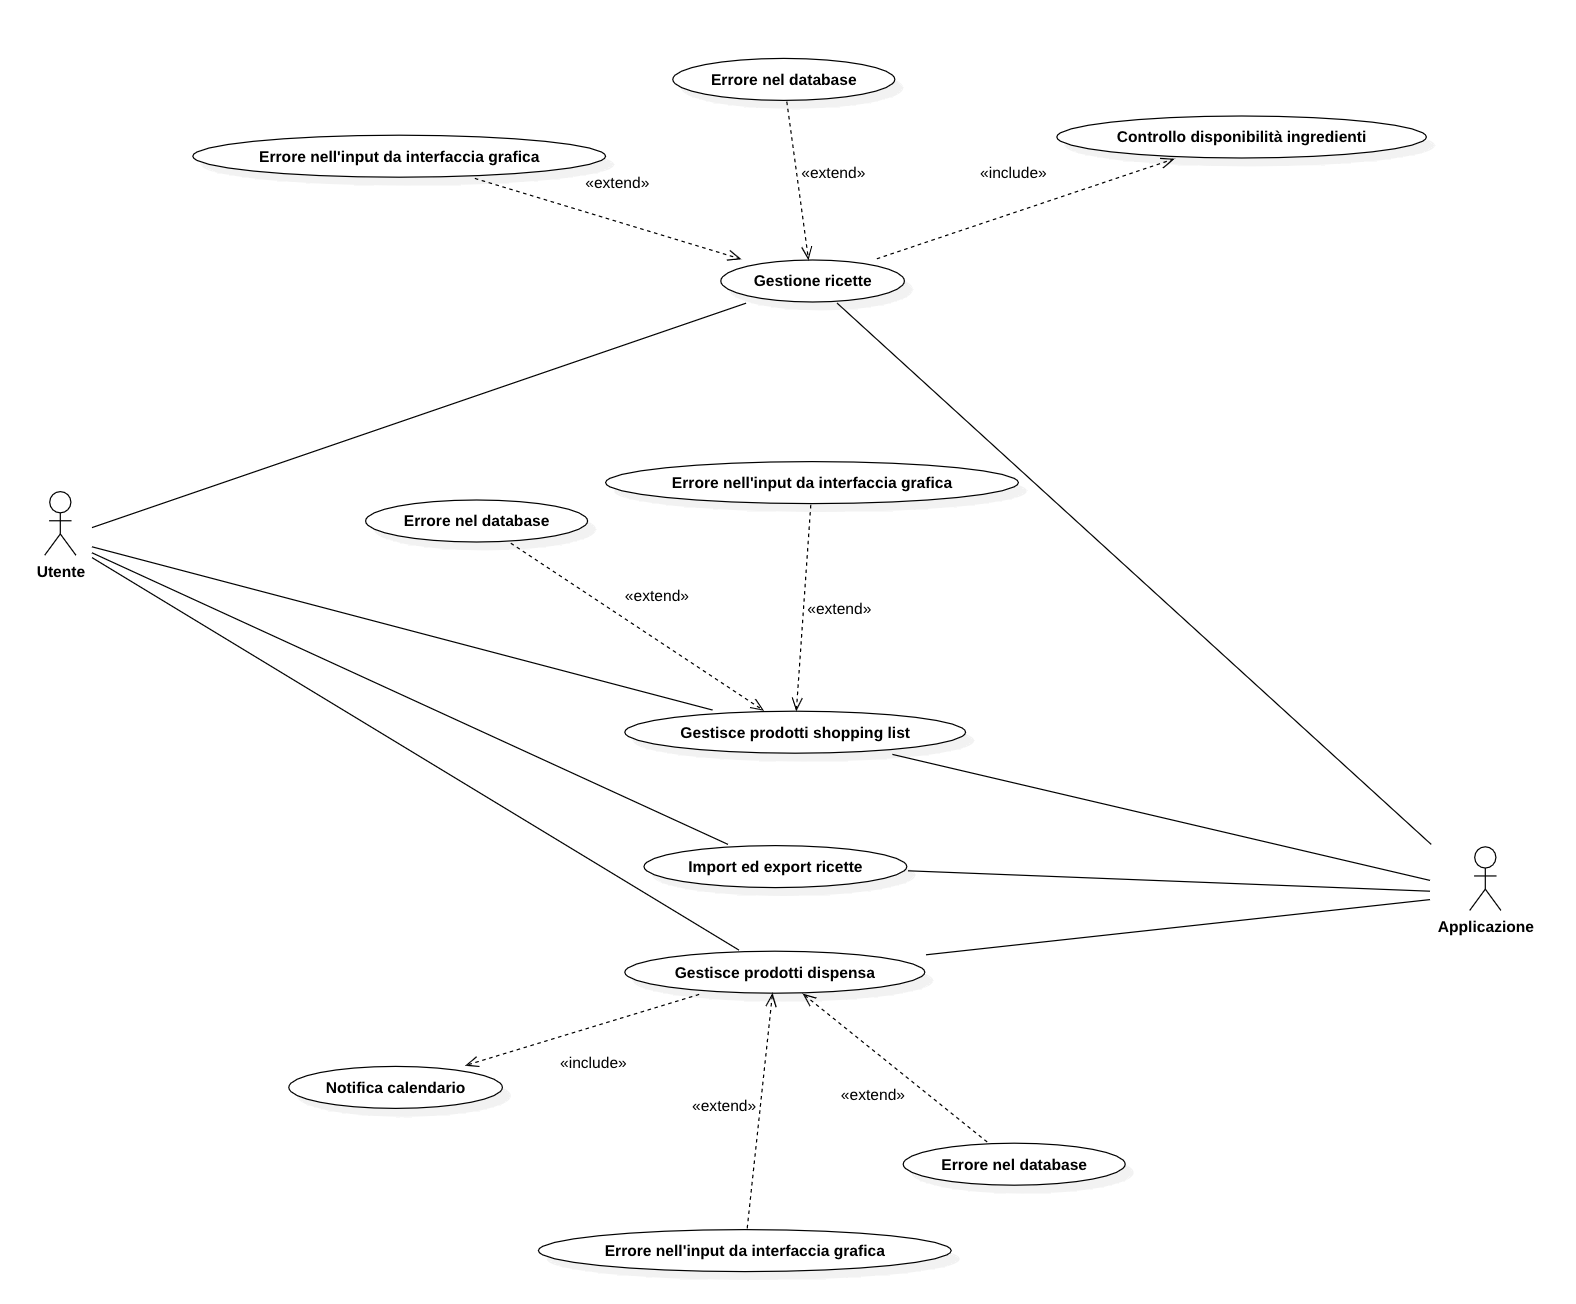
\includegraphics[width=\linewidth]{images/use-case.png}
    \caption{Diagramma dei casi d'uso.}
    \label{fig:usecase}
\end{figure}

\subsection{Activity diagram}

L'activity diagram consente di specificare come il sistema realizzerà le funzionalità mostrate nello use case. Lo scopo è connettere tra loro azioni di alto livello per rappresentare un processo che viene svolto nel sistema. Per una migliore comprensione del funzionamento, nei diagrammi seguenti si è scelto di non modellare i casi di errore del database e dell'interfaccia grafica. 

\subsubsection{Activity diagram della dispensa}

In questo diagramma viene mostrato il processo relativo all'interazione fra l'utente e l'applicazione per la gestione della dispensa. 

\begin{figure}[H]
    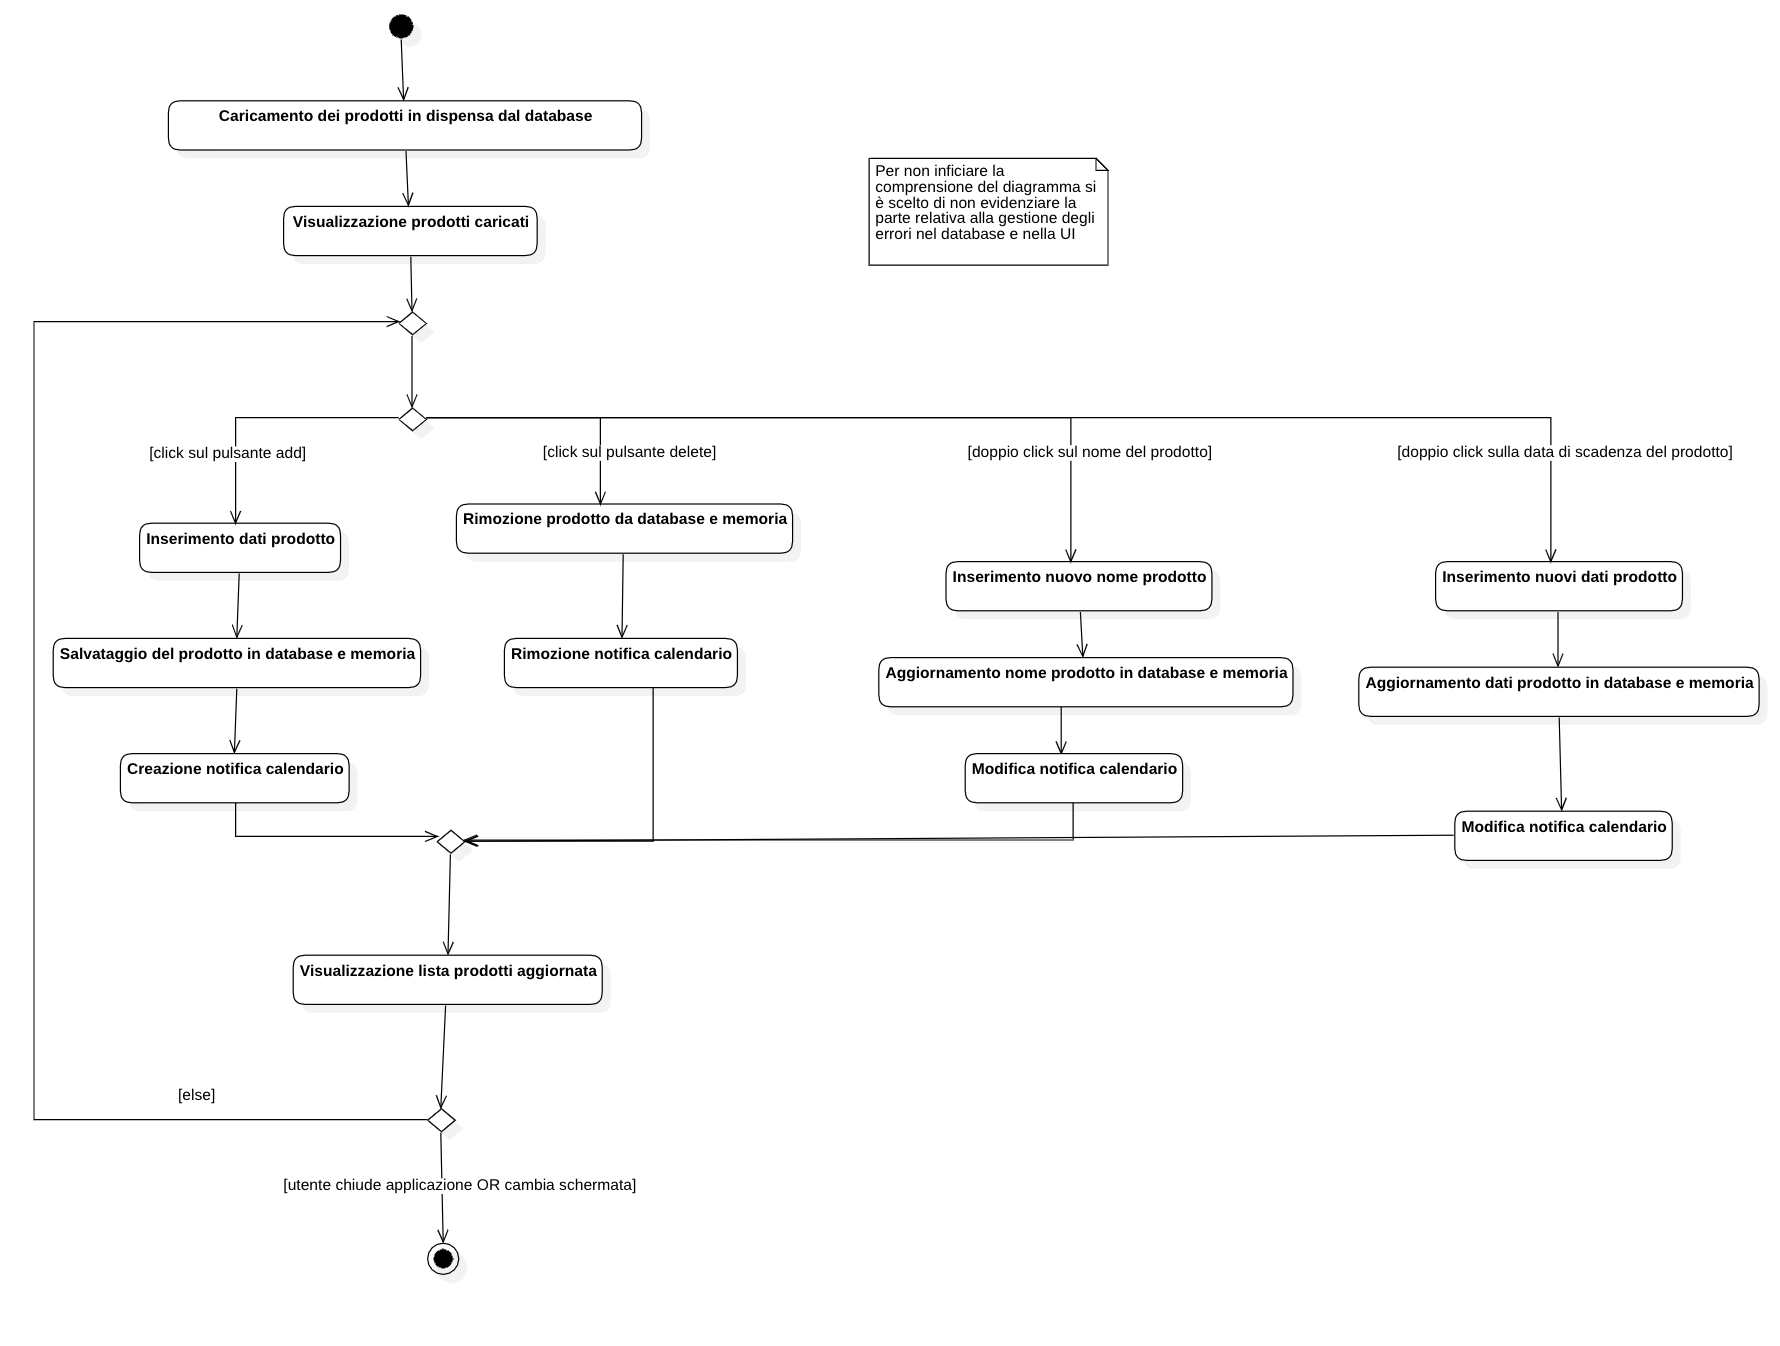
\includegraphics[width=\linewidth]{images/activity-pantry.png}
    \caption{Diagramma delle attività della dispensa.}
    \label{fig:actpantry}
\end{figure}

\subsubsection{Activity diagram della lista della spesa}

In questo diagramma viene mostrato il processo relativo all'interazione fra l'utente e l'applicazione per la gestione della lista della spesa.

\begin{figure}[H]
    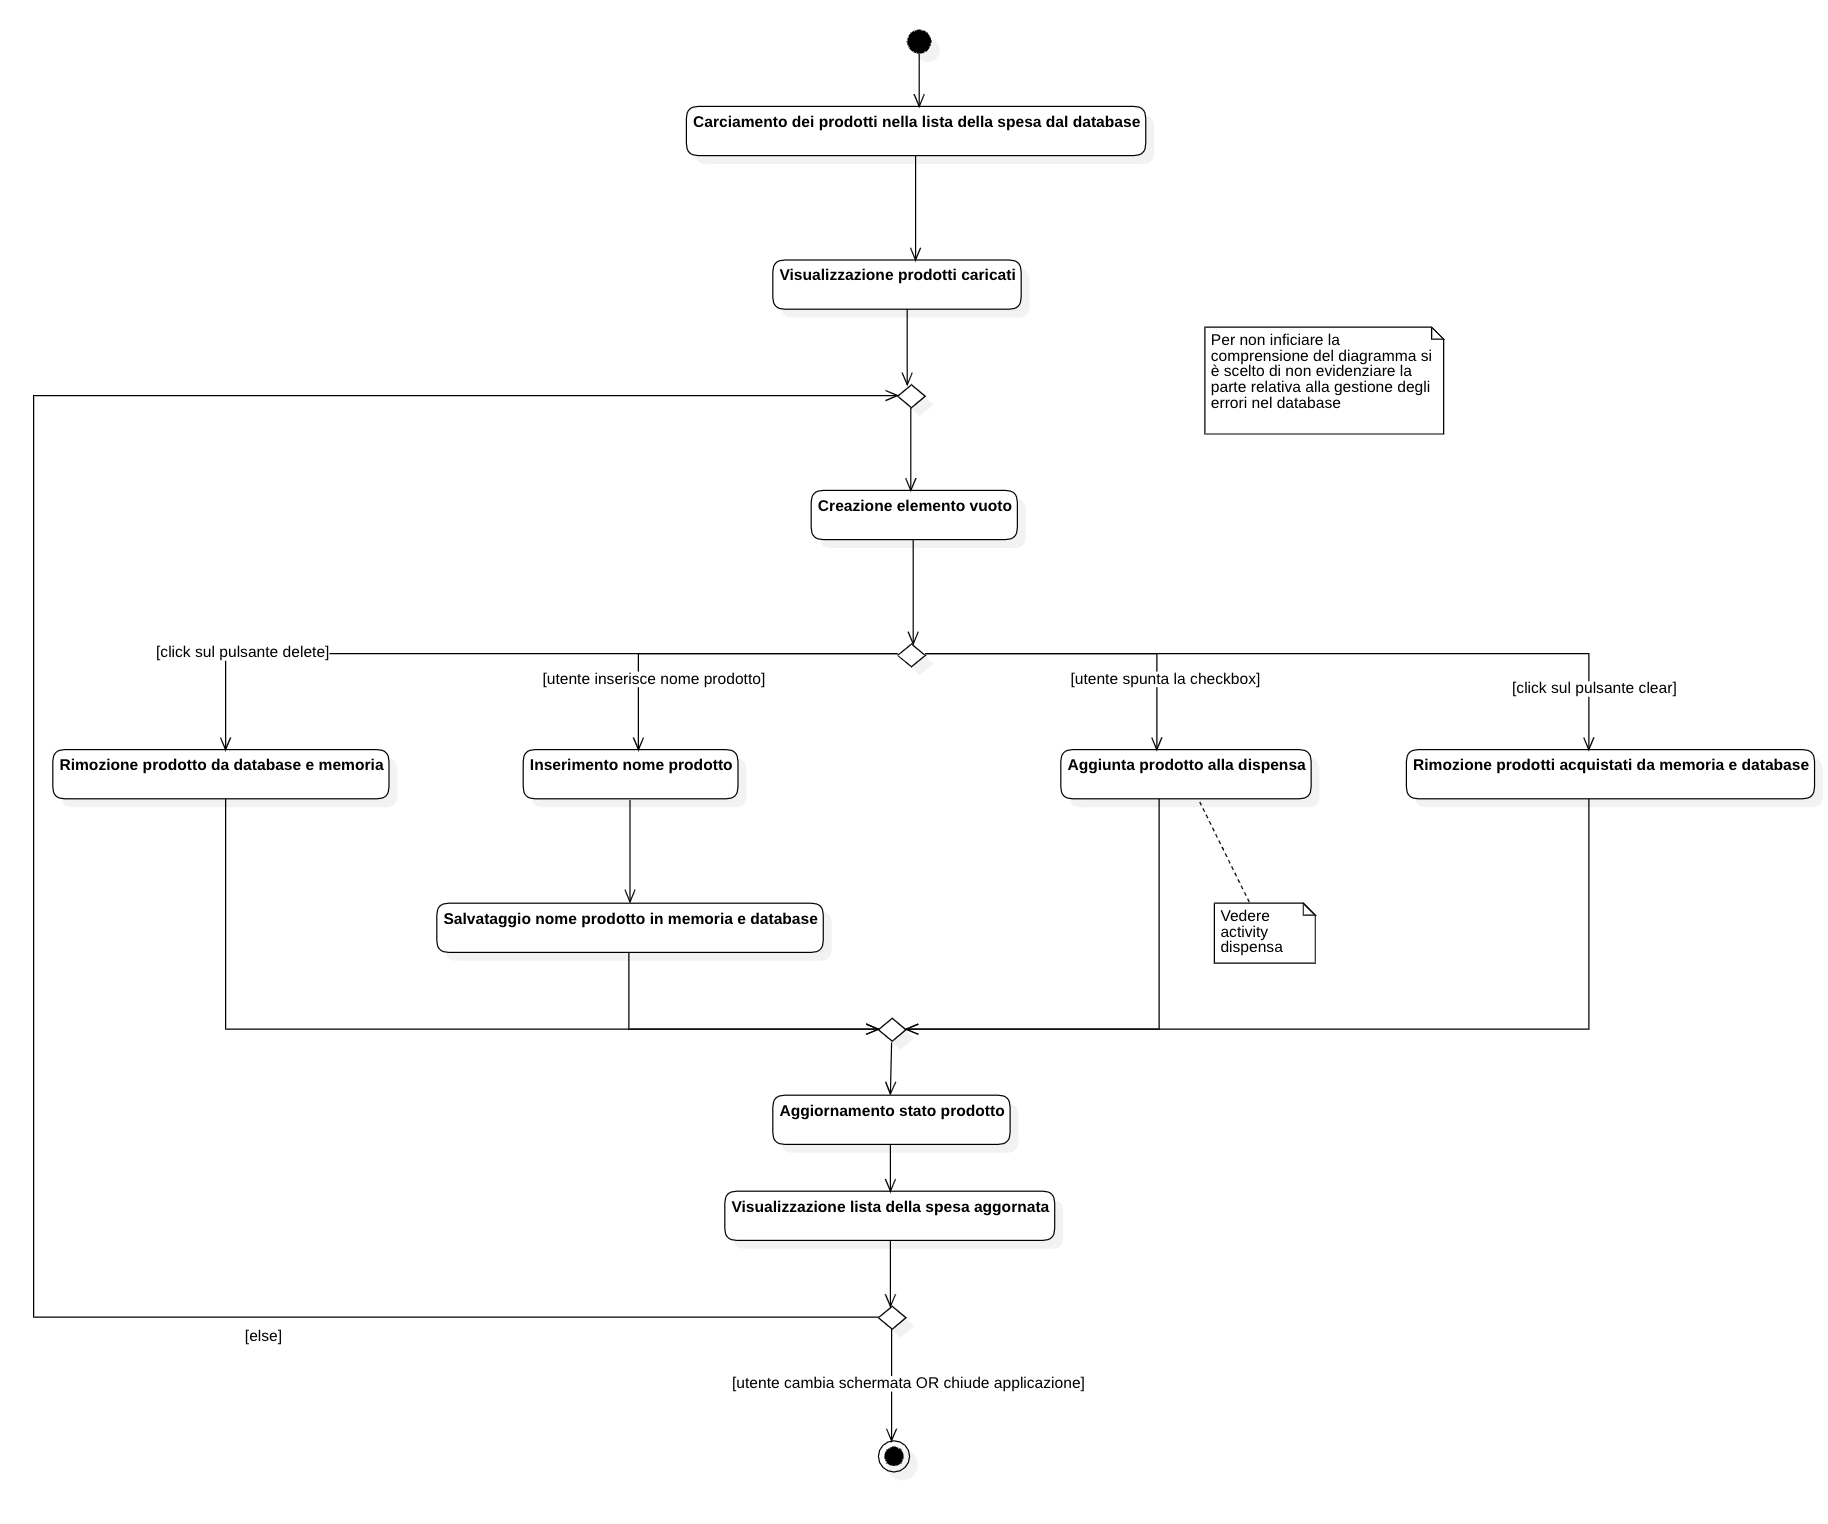
\includegraphics[width=\linewidth]{images/activity-shopping-list.png}
    \caption{Diagramma delle attività della lista della spesa.}
    \label{fig:actshoplist}
\end{figure}

\subsubsection{Activity diagram delle ricette}

In questo diagramma viene mostrato il processo relativo all'interazione fra l'utente e l'applicazione per la gestione delle ricette, inclusa la possibilità di importare ed esportare ricette.

\begin{figure}[H]
    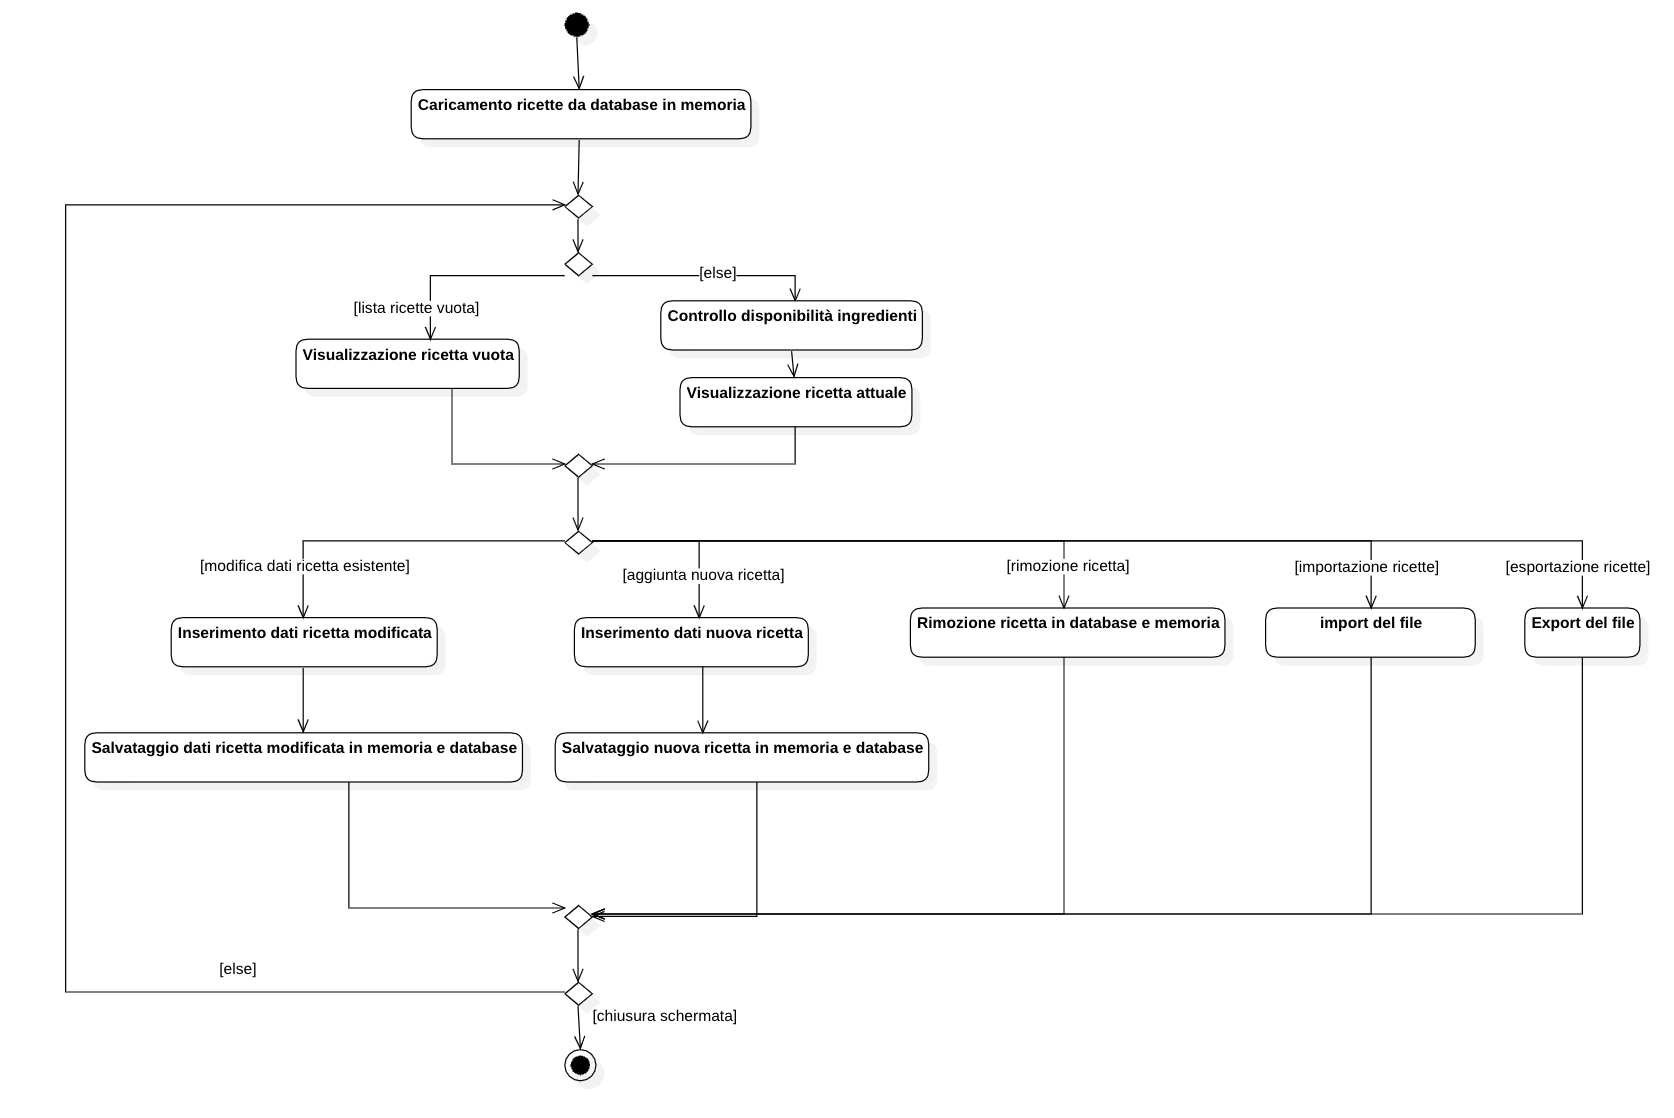
\includegraphics[width=\linewidth]{images/activity-recipe.png}
    \caption{Diagramma delle attività delle ricette.}
    \label{fig:actrecipe}
\end{figure}

\subsection{State diagram}

Lo state diagram permette di modellare gli stati in cui si trova un oggetto e gli eventi che causano le transizioni fra gli stati. 

\subsubsection{State diagram della ricetta}

In questo diagramma vengono mostrati gli stati in cui si può trovare una ricetta in base alla presenza, e alla disponibilità, degli ingredienti.

\begin{figure}[H]
    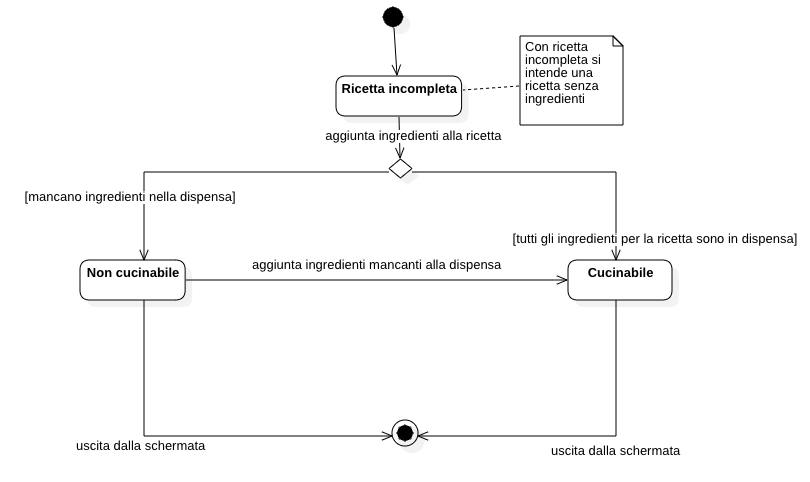
\includegraphics[width=\linewidth]{images/state-recipe.png}
    \caption{Diagramma degli stati della ricetta.}
    \label{fig:staterecipe}
\end{figure}

\subsubsection{State diagram della lista della spesa}

In questo diagramma vengono mostrati gli stati in cui si può trovare un prodotto presente nella lista della spesa.

\begin{figure}[H]
    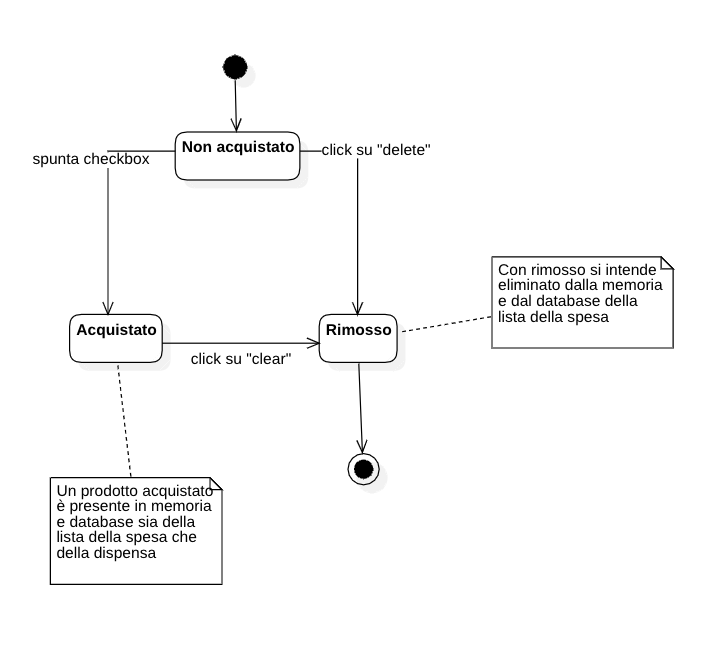
\includegraphics[width=\linewidth]{images/state-shopping-list.png}
    \caption{Diagramma degli stati della lista della spesa.}
    \label{fig:stateshoplist}
\end{figure}

\subsection{Class diagram}

Il class diagram permette di descrivere i tipi di oggetti presenti nel sistema e le relazioni statiche che intercorrono tra di essi. Esso descrive inoltre gli attributi e i metodi di ogni classe, oltre ai vincoli che si applicano nel collegamento tra gli oggetti.

\begin{figure}[H]
    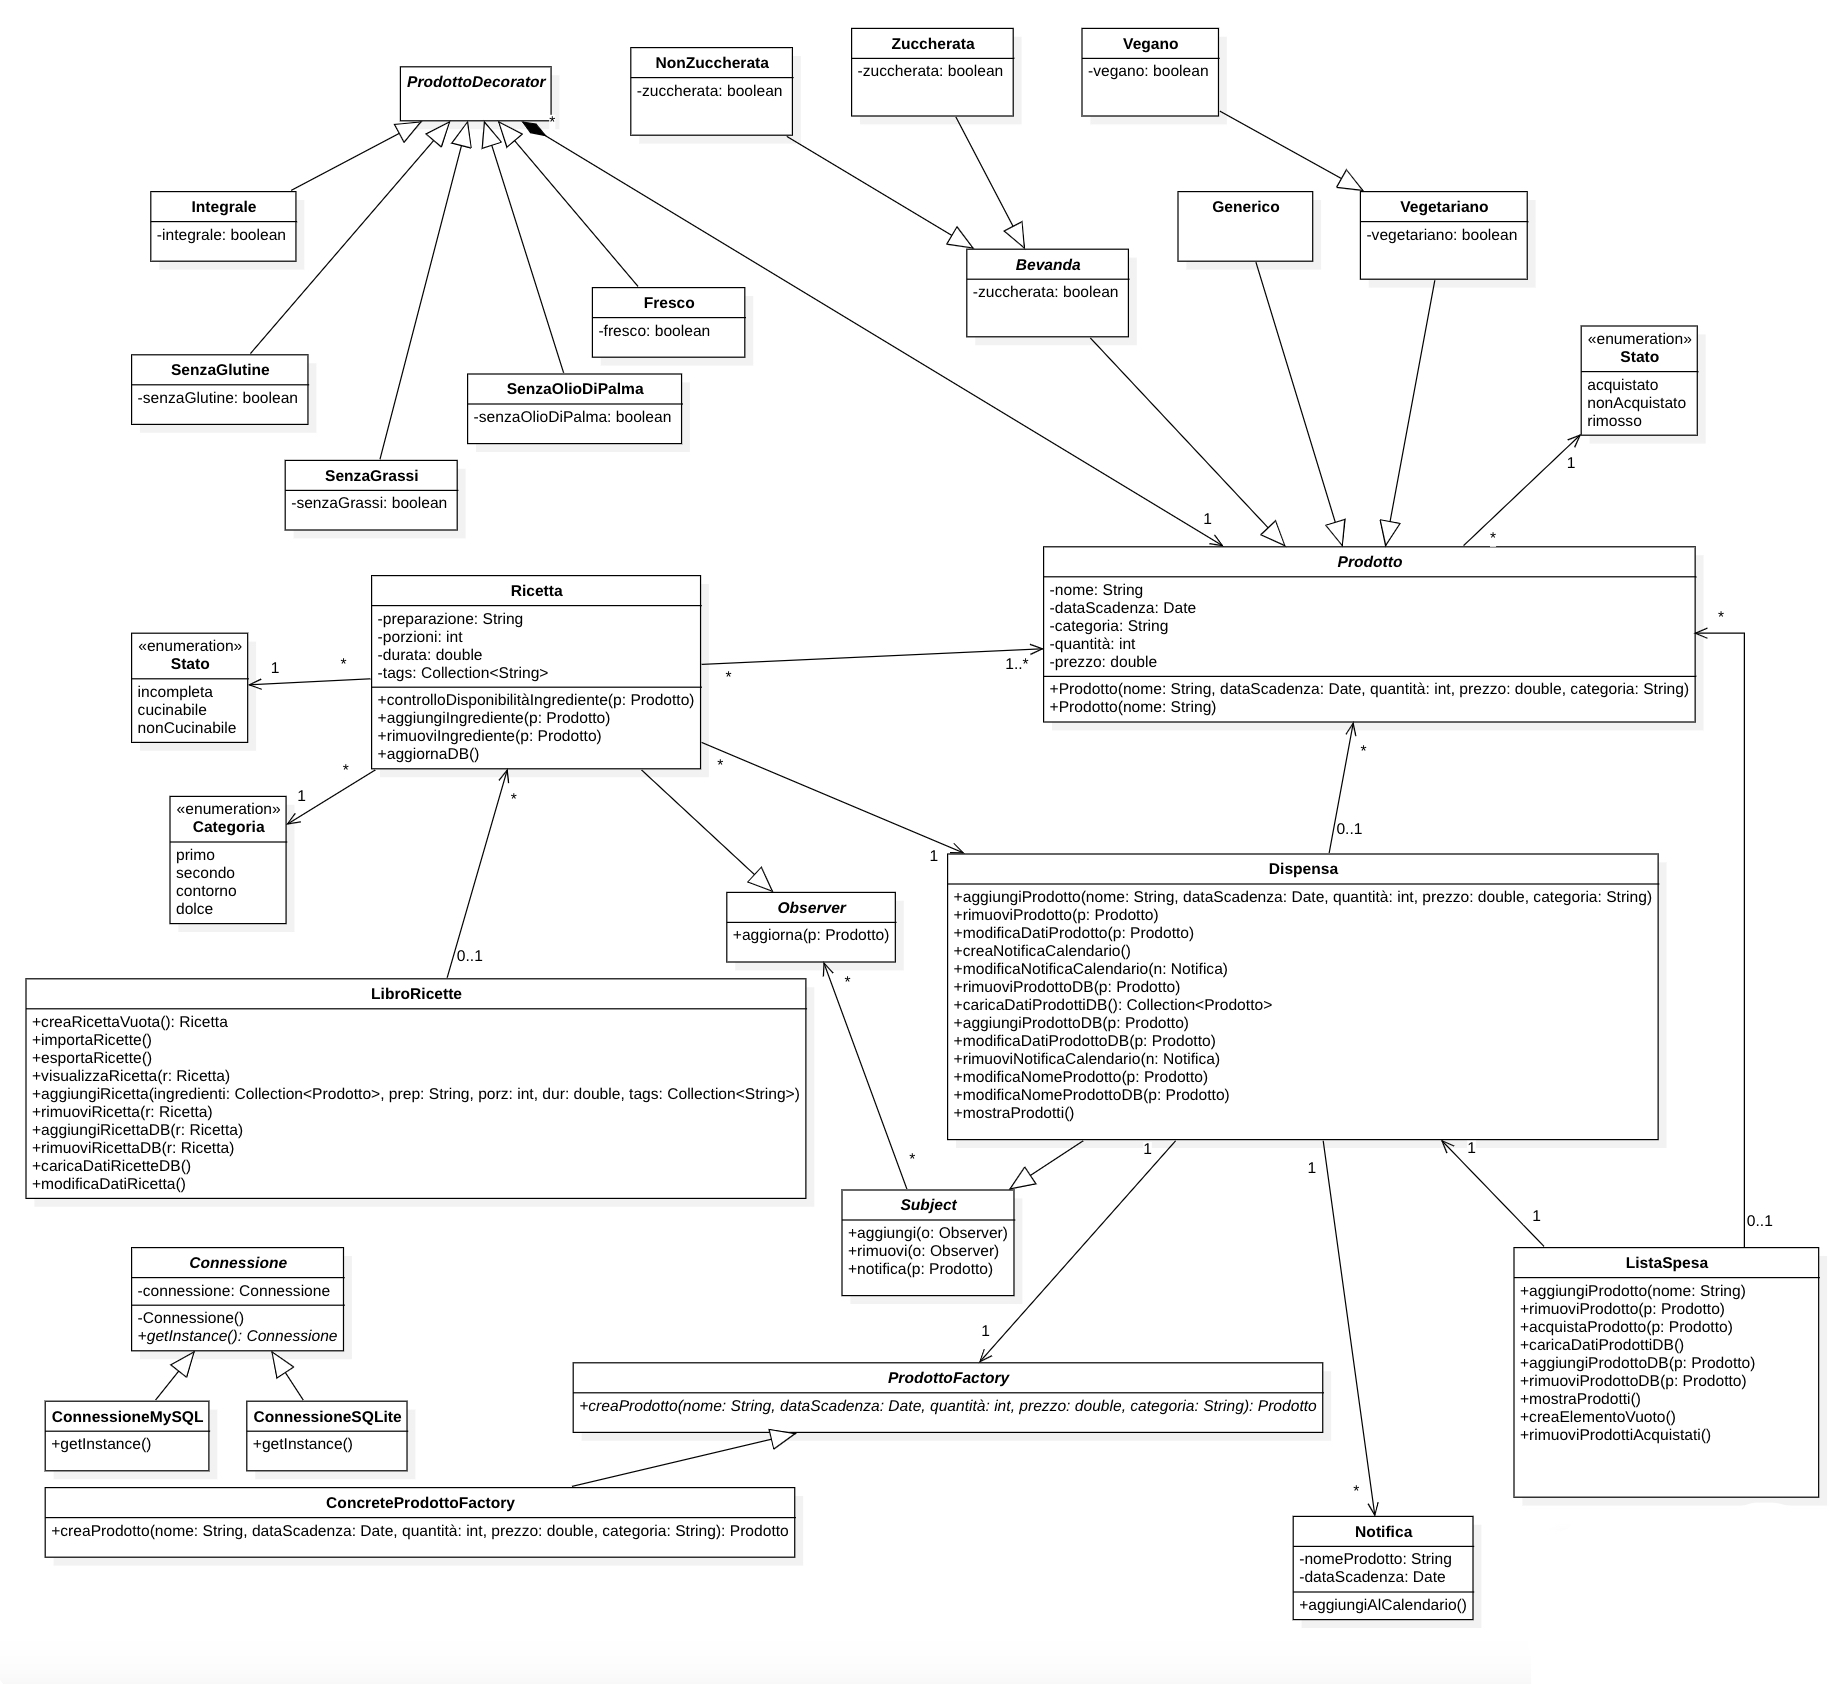
\includegraphics[width=\linewidth]{images/class.jpeg}
    \caption{Diagramma delle classi.}
    \label{fig:classdiagram}
\end{figure}

Per non complicare ulteriormente il diagramma si è scelto di non rappresentare la parte relativa all'interfaccia grafica. I design pattern applicati verranno spiegati nella sezione corrispondente.

\subsection{Sequence diagram}

Il sequence diagram serve per descrivere singoli scenari dell'applicazioni. Lo scopo è mostrare come il sistema svolge le proprie funzioni. Per una migliore comprensione del funzionamento, nei diagrammi seguenti si è scelto di non modellare i casi di errore del database e dell'interfaccia grafica. 

\subsubsection{Sequence diagram della dispensa}

TODO.

\begin{figure}[H]
    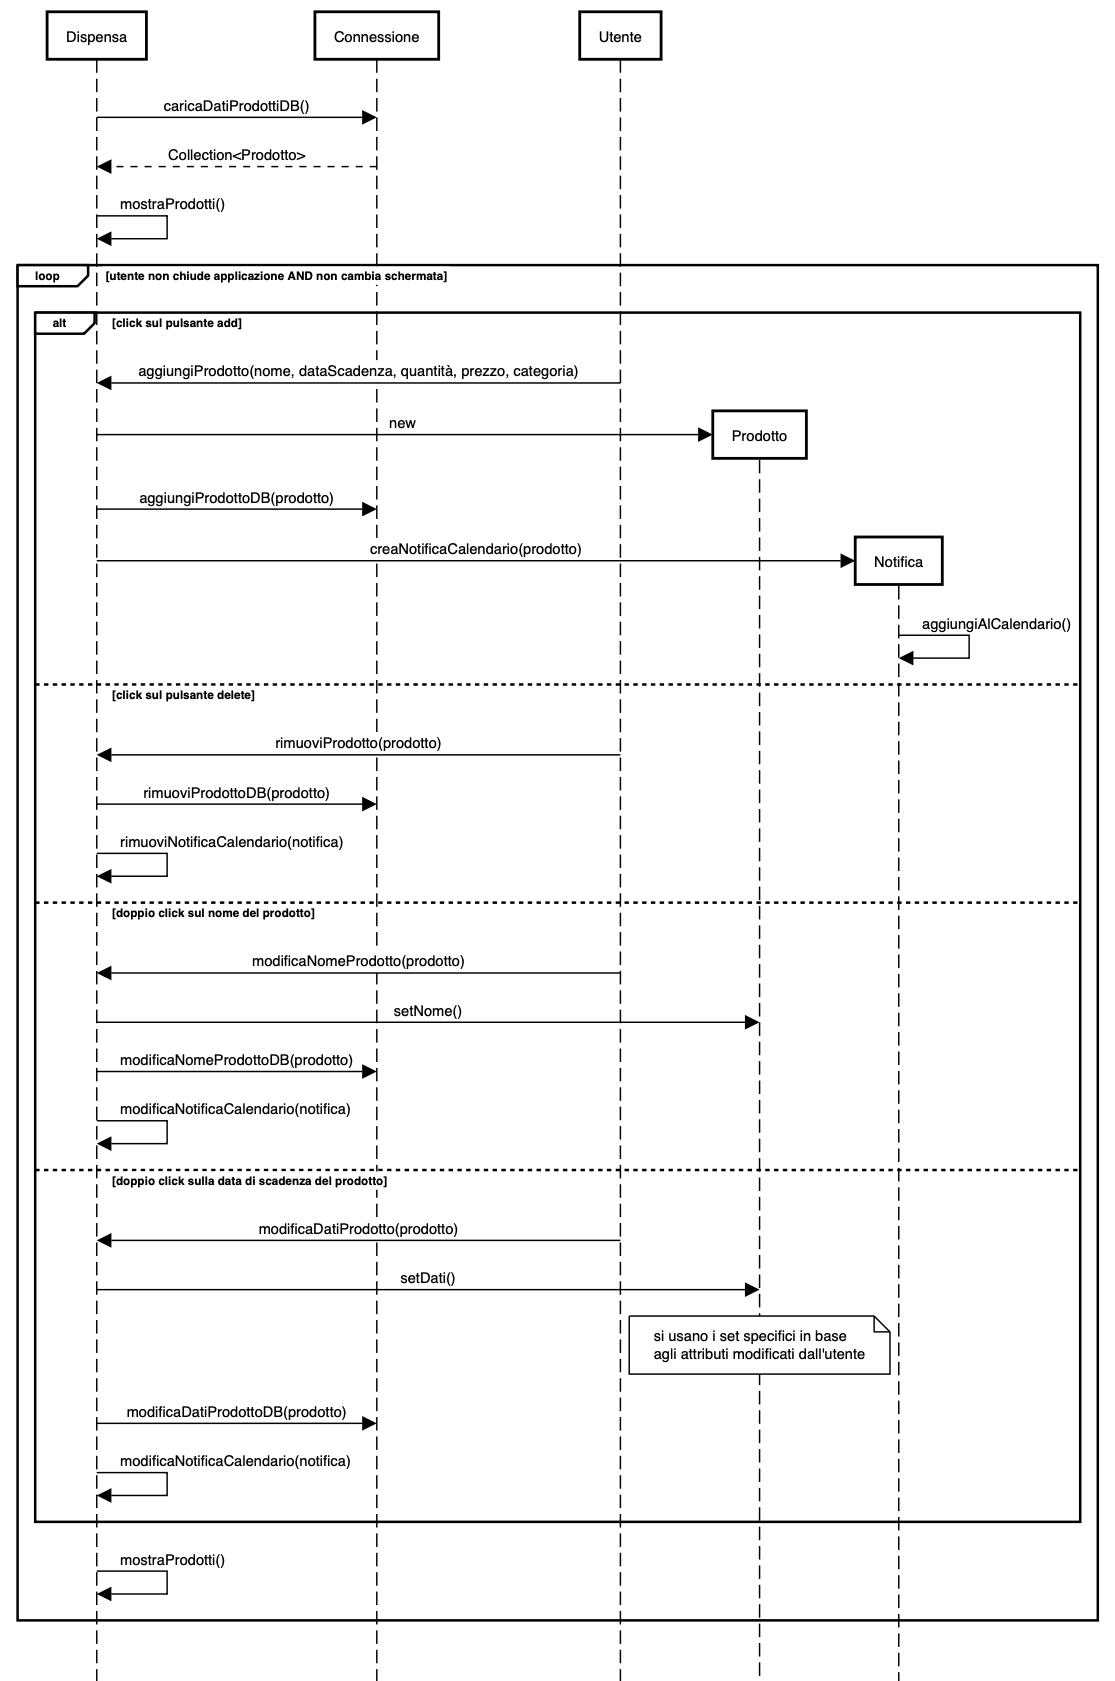
\includegraphics[width=\linewidth]{images/sequence-pantry.png}
    \caption{Diagramma di sequenza della dispensa}
    \label{fig:seqpantry}
\end{figure}

\subsubsection{Sequence diagram della lista della spesa}

TODO.

\begin{figure}[H]
    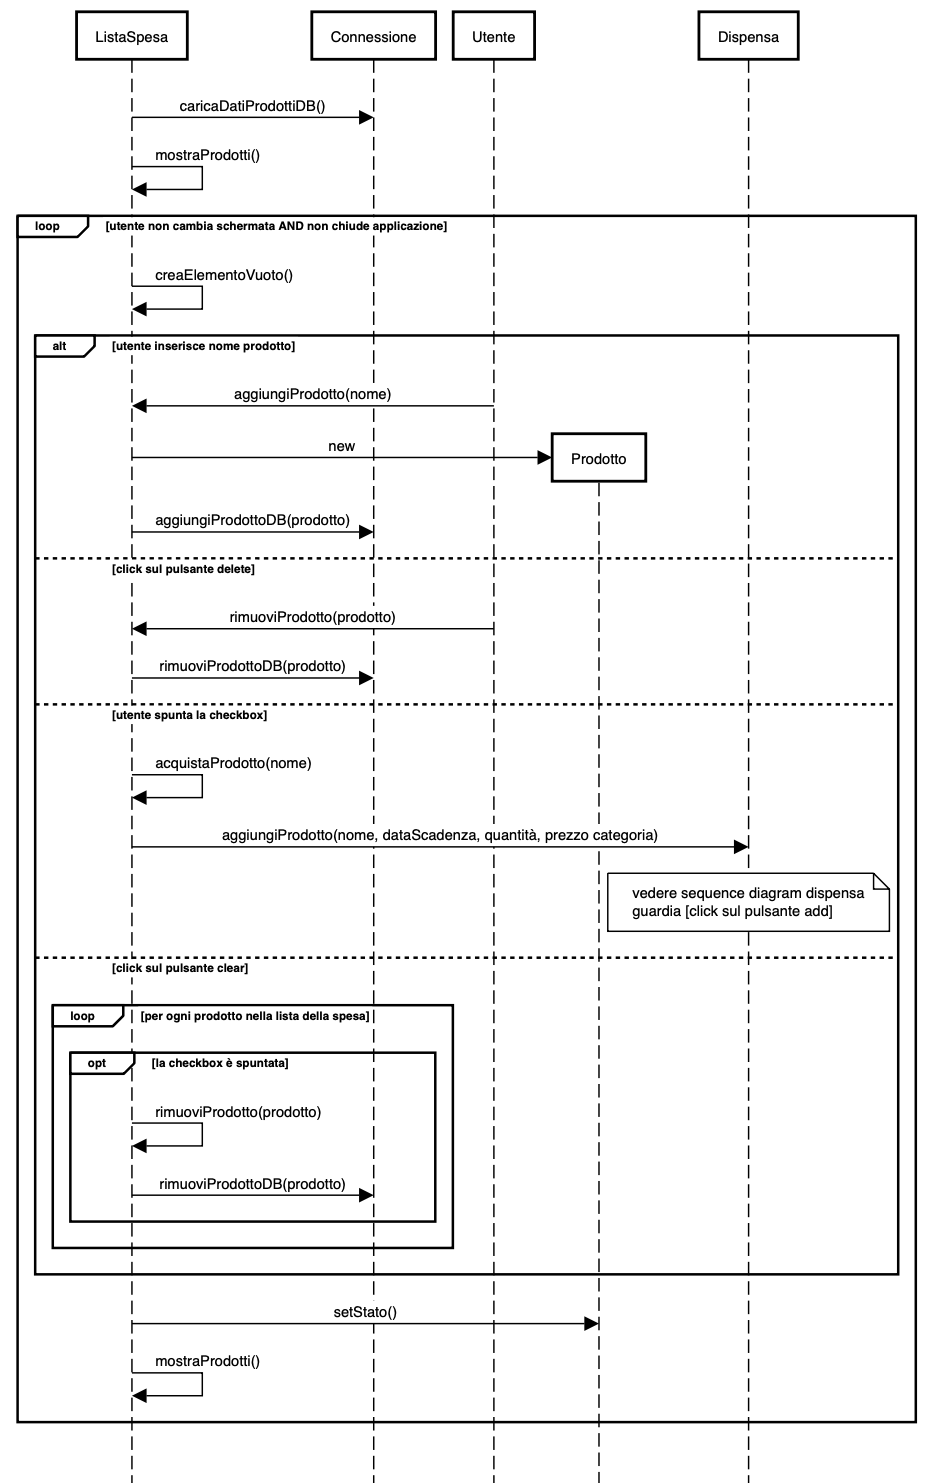
\includegraphics[width=\linewidth]{images/sequence-shopping-list.png}
    \caption{Diagramma di sequenza della lista della spesa}
    \label{fig:seqshoplist}
\end{figure}

\subsubsection{Sequence diagram delle ricette}

Si noti che, per evitare sovrapposizioni nel diagramma che ne avrebbero resa più difficile la comprensione, il metodo \inlinecode{Java}{creaRicettaVuota()} (che si limita a mostrare dei campi di testo vuoti all'utente tramite l'interfaccia grafica) non crea un oggetto di tipo Ricetta (come invece avviene nel caso del metodo \\ \inlinecode{Java}{aggiungiRicetta(ingredienti, preparazione, porzioni, durata, tags)} in cui la ricetta creata presenta valori non nulli nei propri attributi).

\begin{figure}[H]
    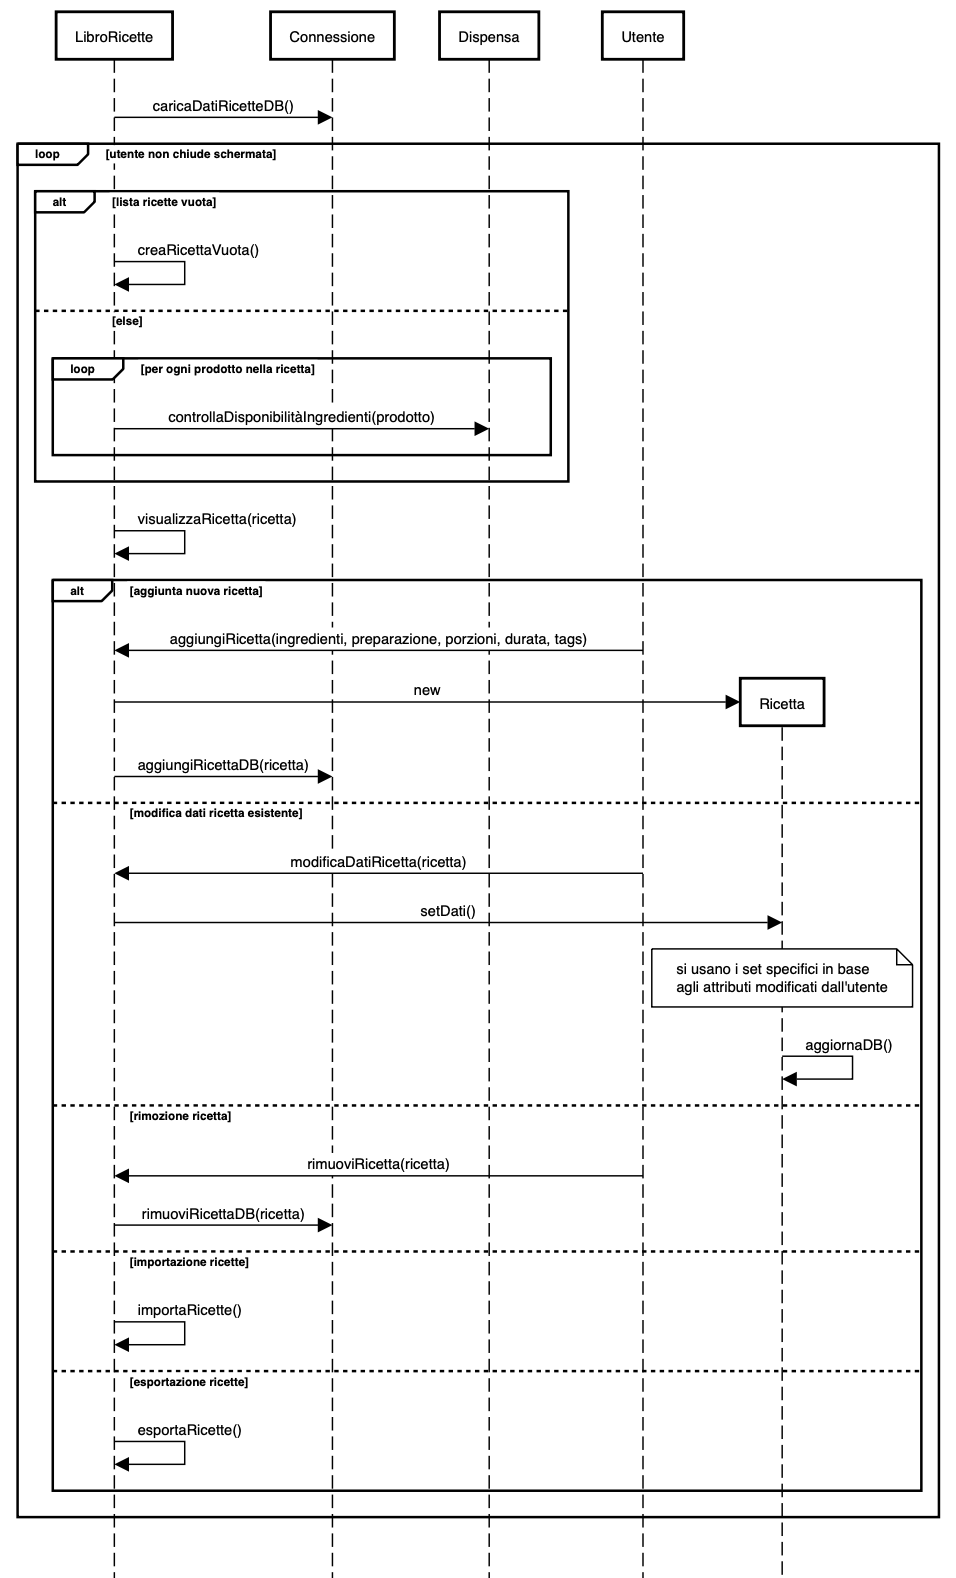
\includegraphics[width=\linewidth]{images/sequence-recipe.png}
    \caption{Diagramma di sequenza delle ricette}
    \label{fig:seqrecipe}
\end{figure}

\section{Design Pattern}

TODO.

\subsection{Factory}

TODO.

\subsection{Iterator}

TODO.

\subsection{Observer}

TODO.

\subsection{Singleton}

TODO.

\subsection{Decorator}

TODO.

\section{ORM}

TODO.

\subsection{Vantaggi}

TODO.

\subsection{Svantaggi}

TODO.

\subsection{Stress test}

TODO.

\begin{appendix}
    \listoffigures
\end{appendix}

\end{document}